\scanpage{14}
\figure{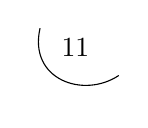
\begin{tikzpicture}[x=1cm,y=1cm]
\node at (0,0) {\mspage{11}};
\draw (-.45,.25) .. controls (-.6,-.4) and (.1,-.65) .. (.55,-.35);
\end{tikzpicture}}
\[
\left\{\begin{aligned}
L\Lambda&=1-\sum_{0\leq i\leq n}\pi_{i,0}\\
\Lambda L&=1-\sum_{n\leq j\leq2n}\pi_{\deleted{2}j,0}
\end{aligned}\right.
\tag{6.15}
\]
\deleted{As for the $\pi_{j,0}$, they are determined by the}

\uline{Question} Give a system of \deleted{\unsure{generators}} relations between the $\Lambda,L$ exclusively, \deleted{\unsure{and}} of relations expressing the $\pi_i$ as polynomials in $L,\Lambda$ .... --- which define $\Lambda$ in terms of $L$ and of the $\pi_i$ ....
\margin{\figure{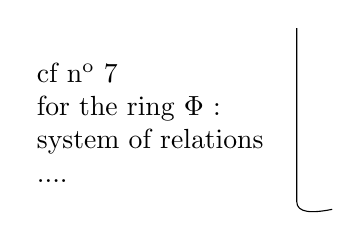
\begin{tikzpicture}[x=1cm,y=1cm]
\node[align=left,text width=3cm] at (0,0) {cf n\textsuperscript{o} 7\\for the ring $\Phi$ :\\system of relations ....};
\draw (1.8,1.2) -- (1.8,-1) .. controls (1.8,-1.15) and (2,-1.15) .. (2.25,-1.1);
\end{tikzpicture}}}

7. Returning to an abstract graded ring $\mathcal E$, equipped with an
\[
L\in\mathcal E^{(2)},
\]
one wants to abstract the preceding situation, without using $M^*$, in terms of the properties of the graded ring \deleted{$\mathcal E$} $\mathcal E^*$ alone equipped with $L\in\mathcal E^{(2)}$.
For this let us start \deleted{from} from a free module $\mathbf M_0$ of rank $2n$ over $\mathbb Z$, equipped with a nondegenerate alternating $2$-form \inserted{\figure{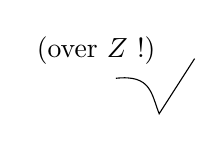
\begin{tikzpicture}[x=1cm,y=1cm]
\node at (0,.25) {(over $\mathbb Z$ !)};
\draw (.25,-.1) .. controls (.7,-.05) and (.7,-.3) .. (.8,-.55) -- (1.25,.15);
\end{tikzpicture}}} $\xi_0\in\bigwedge^2\mathbf M_0$, \inserted{\figure{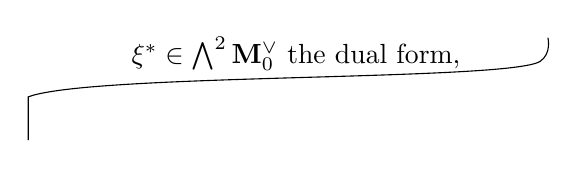
\begin{tikzpicture}[x=1cm,y=1cm]
\node at (0,.3) {$\xi^*\in\bigwedge^2\mathbf M_0^\vee$ the dual form,};
\draw (-3.4,-.8) -- (-3.4,-.25) .. controls (-2.6,.05) and (2.7,-.05) .. (3.1,.2) .. controls (3.25,.3) and (3.2,.5) .. (3.2,.5);
\end{tikzpicture}}} let \deleted{$\xi$} $\mathbf M_0^*=\bigwedge\mathbf M_0$, and let us consider on $\mathbf M_0^*$ the operators
\[
\mathbf Lx=\xi_0x,\qquad\boldsymbol\Lambda_0x=\xi_0^*\mathbin{\lrcorner}x
\]
and let us consider the algebra
\[
\Phi_0=\mathbb Z[\mathbf L_0,\boldsymbol\Lambda_0]\subset\operatorname{End}_{\mathbb Z}(\mathbf M_0^*)
\]
\margin{graded ring.}
Let us note that $\operatorname{End}(\mathbf M_0^*)$, \inserted{\figure{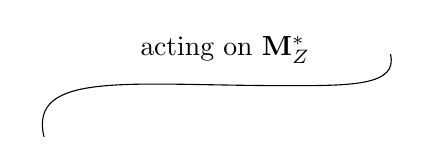
\begin{tikzpicture}[x=1cm,y=1cm]
\node at (0,.35) {acting on $\mathbf M_{\mathbb Z}^*$};
\draw (-2.3,-.75) .. controls (-2.5,.1) and (-1.2,-.1) .. (.8,-.1) .. controls (1.6,-.1) and (2.2,-.1) .. (2.1,.3);
\end{tikzpicture}}} equipped with $\unsure{\mathbf L|\mathbf L_0}$, satisfies the condition of $(6.1)\unsure{(\omega)|(i)|_i}$, \deleted{\unsure{therefore}} and \deleted{$\xi$} $\boldsymbol\Lambda_0$ is the associated operator defined by $(6.5)$.
\mspage{13}
